\documentclass[11pt,american,czech]{article}
\usepackage[a4paper]{geometry}
\geometry{verbose,tmargin=2.5cm,bmargin=2.5cm,lmargin=2cm,rmargin=2cm,headheight=0.8cm,headsep=1cm,footskip=0.5cm}
\setcounter{secnumdepth}{3}
\usepackage{url}
\usepackage{amsmath}
\usepackage{amsthm}
\usepackage{amssymb}
\usepackage{graphicx}
\usepackage{setspace}
\usepackage{enumerate} %roman enumiration
\usepackage{threeparttable}
\usepackage{algorithmic}
\usepackage{algorithm}
\usepackage{array}
\usepackage[utf8]{inputenc} % Required for inputting international characters
\usepackage[T1]{fontenc} % Output font encoding for international characters
\usepackage{mathpazo} % Palatino font

\makeatletter
%%%%%%%%%%%%%%%%%%%%%%%%%%%%%% Algorithms
% Define a \HEADER{Title} ... \ENDHEADER block
\newcommand{\HEADER}[1]{\ALC@it\underline{\textsc{#1}}\begin{ALC@g}}
	\newcommand{\ENDHEADER}{\end{ALC@g}}
\renewcommand*{\ALG@name}{Algoritmus}
\algsetup{indent=2em} 
\renewcommand{\algorithmiccomment}[1]{\hspace{2em}// #1} 
\makeatother

%% Use Times New Roman font for text and Belleek font for math
%% Please make sure that the 'esint' package is turned off in the
%% 'Math options' page.
\usepackage[varg]{txfonts}


%% Indent even the first paragraph in each section
\usepackage{indentfirst}

% completely avoid orphans (first lines of a new paragraph on the bottom of a page)
\clubpenalty=9500

% completely avoid widows (last lines of paragraph on a new page)
\widowpenalty=9500

% disable hyphenation of acronyms
\hyphenation{CDFA HARDI HiPPIES IKEM InterTrack MEGIDDO MIMD MPFA DICOM ASCLEPIOS MedInria}

%%---------------------------------------------------------------------

%% Print out all vectors in bold type instead of printing an arrow above them
%%\renewcommand{\vec}[1]{\boldsymbol{#1}}

% Replace standard \cite by the parenthetical variant \citep
%\renewcommand{\cite}{\citep}

\makeatother
\pagestyle{empty} %turns off page numbering
\usepackage{babel}
\newcommand*\Laplace{\mathop{}\!\mathbin\bigtriangleup}
\newcommand*\midpoint[1]{\overline{#1}}

\begin{document}
\selectlanguage{czech}
\def\documentdate{...}


\begin{titlepage} % Suppresses displaying the page number on the title page and the subsequent page counts as page 1
	\newcommand{\HRule}{\rule{\linewidth}{0.5mm}} % Defines a new command for horizontal lines, change thickness here
	\center % Centre everything on the page	
	
	\textsc{\LARGE FJFI ČVUT}\\[1.5cm] % Main heading such as the name of your university/college
	\vfill
%	
\includegraphics[width=0.2\textwidth]{Images/TITLE/fjfi}\\[1cm] % Include a department/university logo - this will require the graphicx package	
	
%	\noindent %
%	\begin{minipage}[c]{3cm}%
%		\noindent \begin{center}
%			
\includegraphics[width=3cm,height=3cm,keepaspectratio]{Images/TITLE/cvut}
%			\par\end{center}%
%	\end{minipage}%
%	\begin{minipage}[c]{0.6\linewidth}%
%		\begin{center}
%			\textsc{\large{}České vysoké učení technické v Praze}{\large{}}\\
%			{\large{}Fakulta jaderná a fyzikálně inženýrská}
%			\par\end{center}%
%	\end{minipage}%
%	\begin{minipage}[c]{3cm}%
%		\noindent \begin{center}
%		
\includegraphics[width=3cm,height=3cm,keepaspectratio]{Images/TITLE/fjfi}
%		\par\end{center}%
%	\end{minipage}
%	\vspace{3cm}
	
	\textsc{\Large Metoda Monte Carlo}\\[0.5cm] % Major heading such as course name
	\textsc{\large Seminární práce}\\[0.5cm] % Minor heading such as course title
	\HRule\\[0.4cm]
	{\huge\bfseries Parabolická evoluční úloha ve 2D}\\[0.4cm] % Title of your document
	\HRule\\[1.5cm]
	{\large\textit{Autor}}\\
	Vladislav \textsc{Belov}\\
	\vfill\vfill\vfill\vfill\vfill\vfill\vfill % Position the date 3/4 down the remaining page
	{\large\today} % Date, change the \today to a set date if you want to be precise
	
	%------------------------------------------------
	%	Logo
	%------------------------------------------------
	
%	\vfill\vfill
%	
\includegraphics[width=0.2\textwidth]{Images/TITLE/fjfi}\\[1cm] % Include a department/university logo - this will require the graphicx package
%	
	%----------------------------------------------------------------------------------------
	
	\vfill % Push the date up 1/4 of the remaining page
	
\end{titlepage}


\section{Úvod}\label{sec:1}

Znalosti způsobů řešení různých diferenciálních rovnic je podstatná pro každého, kdo je aspoň nějak spojen s vědou a technikou. Tato seminární práce se zabývá řešením parabolické diferenciální rovnice popisující vedení tepla ve dvou dimenzích pomocí metody Monte Carlo.

\medskip

Obecně parabolická evoluční úloha ve 2D  na oblasti $(0,T)\times\Gamma$, kde $T\in\mathbb{R}_{+}$ a $\Gamma\subset\mathbb{R}^{2}$, vypadá následovně:

\begin{equation} \label{ini_problem}
	\begin{split}
		\frac{\partial}{\partial t}u(t,x)-D\cdot\Laplace u(t,x)&=f(t,x) ,\\
		u\arrowvert_{\partial\Gamma}&=g(x),\\
		u(0,x)&=h(x).
	\end{split}
\end{equation}
\noindent 
V dané notaci funkce $u=u(t,x)$ popisuje rozložení teploty na oblasti $\Gamma$ (tj. $x\in\Gamma\subset\mathbb{R}^{2}$) v časech $t\in(0,T)$, $D$ je termální difuzivita ($D>0$), $g=g(x)$ je okrajová podmínka evoluční úlohy $\forall t\in(0,T)$ a $h=h(x)$ je počáteční podmínka. V rámci této seminární práce položíme pravou stranu $f\equiv 0$.

\section{Diskretizace úlohy}\label{sec:2}

V numerické matematice se podobné úlohy řeší pomocí metody konečných diferencí (metody sítí), která spočívá v diskretizaci oblasti $(0,T)\times\Gamma$ a konstrukci diferenčního schématu (viz \cite{BENES2017}). Pro jednoduchost budeme hledat řešení úlohy \eqref{ini_problem} na čtverci $\Gamma=(-b,b)\times(-b,b)$, $b>0$, pak lze definovat na uzavřeném čtverci $\midpoint{\Gamma}$ čtvercovou síť $\midpoint{\omega}_{h}$ s krokem $h>0$, tj. $\Gamma\leftrightarrow\omega_{h}$ a $\partial\Gamma\leftrightarrow\midpoint{\omega}_{h}\setminus\omega_{h}$. Potom, rozdělíme-li interval $[0,T]$ na časové hladiny s krokem $\tau=\tfrac{T}{N_{T}}$, kde $N_{T}$ je počet hladin, a označíme-li $u^{\,k}_{i,j}$ hodnoty funkce $u$ na časových hladinách $k\in\{0,1,\dots,N_{T}\}$ pro všechny $(i,j)$ body sítě $\midpoint{\omega}_{h}$, dostaneme podle \cite{BENES2017} následující diferenční schéma:

\begin{equation} \label{fin_diff_scheme}
	\begin{split}
		\frac{u^{\,k+1}_{i,j}-u^{\,k}_{i,j}}{\tau}=D\cdot\big(\frac{u^{\,k}_{i+1,\,j}-2u^{\,k}_{i,j}+u^{\,k}_{i-1,\,j}}{h^{2}}&+\frac{u^{\,k}_{i,\,j+1}-2u^{\,k}_{i,j}+u^{\,k}_{i,\,j-1}}{h^{2}}\big),\,\forall(i,j)\in\omega_{h},\,\forall k\in\{0,1,\dots,N_{T}-1\};\\	
		u^{\,k}_{i,j}&=g_{i,j},\forall(i,j)\in\midpoint{\omega}_{h}\setminus\omega_{h},\,\forall k\in\{0,1,\dots,N_{T}\};\\
		u^{\,0}_{i,j}&=h_{i,j},\,\forall(i,j)\in\midpoint{\omega}_{h}.
	\end{split}
\end{equation}

Takovému-to diferenčnímu schématu se říká \textit{explicitní} a jeho chyba aproximace je $O(\tau+h^{2})$. Budeme-li volit kroky $\tau$ a $h$ v poměru $\frac{h^{2}}{\tau}=4$ a položíme-li $D=1$, pak \eqref{fin_diff_scheme} se přepíše následovně:

\begin{equation}\label{final_fin_diff_scheme}
	\begin{split}
		u^{\,k}_{i,j}=\frac{1}{4}\big(u^{\,k-1}_{i+1,\,j}+u^{\,k-1}_{i-1,\,j}&+u^{\,k-1}_{i,\,j+1}+u^{\,k-1}_{i,\,j-1}\big),\,\forall(i,j)\in\omega_{h},\,\forall k\in\{0,1,\dots,N_{T}-1\};\\
		u^{k}_{i,j}&=g_{i,j},\forall(i,j)\in\midpoint{\omega}_{h}\setminus\omega_{h},\,\forall k\in\{0,1,\dots,N_{T}\};\\
		u^{\,0}_{i,j}&=h_{i,j},\,\forall(i,j)\in\midpoint{\omega}_{h}.
	\end{split}
\end{equation}

Stojí za zmínění, že schéma \eqref{final_fin_diff_scheme} je stabilní, neboť podmínka stability pro \eqref{fin_diff_scheme} má tvar: 

\begin{equation*}
	\frac{1}{2}\geq D\cdot\frac{\tau}{h^{2}}.
\end{equation*}

Získanou soustavu lineárních algebraických rovnic budeme řešit pomocí metody Monte Carlo.

\section{Algoritmus výpočtu aproximace}\label{sec:3}

Postup pro řešení soustavy rovnic \eqref{final_fin_diff_scheme} získané diskretizací úlohy \eqref{ini_problem} je velmi jednoduchý - použijeme lehce upravenou náhodnou procházku. Aproximaci $u^{\,k_{0}}_{ij}$ pro jistou pevnou časovou hladinu $k_{0}\in\{0,1,\dots,N_{T}\}$ dostaneme jako výběrovou střední hodnotu jisté náhodné veličiny $Y_{W_{ini}}$ definované následujícím způsobem (\cite{VIRIUS2010}):

\begin{enumerate}
	\item označíme počáteční bod náhodné procházky $W_{ini}=(i,j)\in\omega_{h}$, který se nachází na časové hladině $k_{0}$;
	\item z bodu $W_{ini}$ přejde náhodná procházka s pravděpodobností $\frac{1}{4}$ do libovolného sousedního bodu, který je na časové hladině $k_{0}-1$;
	\item pokud je náhodná procházka stále ve vnitřním bodě sítě $\midpoint{\omega}_{h}$ a není na nulové časové hladině, vrátíme se na krok 2, jinak jdeme na krok 4;
	\item označíme-li $W_{fin}$ bod sítě, ve kterém se nachází náhodná procházka v daném okamžiku, pak definujeme náhodnou veličinu $Y_{W_{ini}}$ takto:
	\begin{itemize}
		\item $Y_{W_{ini}}=h(W_{fin})$, pokud $W_{fin}\in\omega_{h}$, ale $W_{fin}\notin\midpoint{\omega}_{h}$;
		\item $Y_{W_{ini}}=g(W_{fin})$, pokud $W_{fin}\in\midpoint{\omega}_{h}\setminus\omega_{h}$.
	\end{itemize}
\end{enumerate}

Zopakujeme-li tento postup pro všechny body $(i,j)\in\omega_{h}$, dostaneme aproximaci\footnote{Ve zdroji \cite{VIRIUS2010} lze nalézt důkaz toho, že střední hodnoty $Y_{W}$ pro všechna $W$ řeší soustavu rovnic \eqref{final_fin_diff_scheme}.} řešení diferenčního schématu \eqref{final_fin_diff_scheme}.

Označíme-li $\hat{\mu}$ výběrovou střední hodnotu náhodné veličiny $Y_{W}$ pro všechna $W$ a $\hat{s}^{2}$ její výběrový rozptyl, potom chybu $\delta$ vypočítané aproximace nalezneme pomocí vzorce, který přímo vyplývá z Čebyševovy nerovnosti:

\begin{equation}
	\delta=\arrowvert EY_{W}-\hat{\mu}\arrowvert=\sqrt{\frac{\hat{s}^{2}}{N\cdot\varepsilon}},
\end{equation}

\noindent
kde $N$ je počet simulací v rámci metody Monte Carlo (tzn. $N\equiv$ počet náhodných procházek vycházejících z bodu $W$ sítě $\omega_{h}$) a $0<\varepsilon<1$ je hladina významnosti.

\section{Implementace}\label{sec:4}

Součástí této seminární práce je také implementace v programovacím jazyce Matlab, která se skládá z čtyř souborů. Tři z nich obsahují definice funkcí, jež budou popsány podrobněji v následujících podsekcích. V čtvrtém souboru \texttt{main.m} lze nalézt pouze vyvolání řešiče rovnice vedení tepla, který je implementován v \texttt{parabolicPDESolver.m}.

\subsection{Funkce \texttt{parabolicPDESolver}}\label{sec:4.1}

Tato funkce odpovídá za výpočet aproximace řešení diferenčního schématu \eqref{fin_diff_scheme} podle algoritmu popsaného v sekci~\ref{sec:3}.

\begin{itemize}
	\item Vstupní parametry:
		\begin{itemize}
			\item \texttt{numOfSim} - číslo simulací v rámci metody Monte Carlo;
			\item \texttt{b} - číslo $b>0$ určující oblast $\Gamma=(-b,b)\times(-b,b)$;
			\item \texttt{meshStep} - krok $h$ sítě $\midpoint{\omega}_{h}$;
			\item \texttt{maxTime} - časová hladina $k_{0}$, pro niž hledáme aproximaci řešení;
			\item \texttt{verbose} - parametr podrobného výpisu.
		\end{itemize}
	\item Výstupní parametry:
		\begin{itemize}
			\item \texttt{solution} - hledaná aproximace řešení \eqref{final_fin_diff_scheme};
			\item \texttt{solutionErr} - chyba aproximace.
		\end{itemize}
\end{itemize}

\subsection{Funkce \texttt{meshRandomWalk}}\label{sec:4.2}

Tato funkce odpovídá za simulaci náhodné procházky na síti $\midpoint{\omega}_{h}$ definované v sekci~\ref{sec:2}.

\begin{itemize}
	\item Vstupní parametry:
	\begin{itemize}
			\item \texttt{xStartPos} - x-ová souřadnice bodu $W_{ini}$;
			\item \texttt{yStartPos} - y-ová souřadnice bodu $W_{ini}$;
			\item \texttt{meshStep} - analogický význam jako v podsekci~\ref{sec:4.1};
			\item \texttt{b} - analogický význam jako v podsekci~\ref{sec:4.1};
			\item \texttt{maxTime} - analogický význam jako v podsekci~\ref{sec:4.1};
	\end{itemize}
	\item Výstupní parametry:
	\begin{itemize}
			\item \texttt{xFinPos} - x-ová souřadnice bodu $W_{fin}$;
			\item \texttt{yFinPos} - y-ová souřadnice bodu $W_{fin}$.
	\end{itemize}
\end{itemize}

\subsection{Funkce \texttt{calcStats}}\label{sec:4.3}

Tato funkce odpovídá za výpočet statistických vlastností náhodné veličiny $Y_{W}$ definované v sekci~\ref{sec:3}.

\begin{itemize}
	\item Vstupní parametry:
	\begin{itemize}
		\item \texttt{rv} - vektor hodnot náhodné veličiny $Y_{W}$;
		\item \texttt{signLvl} - hladina významnosti;
		\item \texttt{verbose} - parametr podrobného výpisu.
	\end{itemize}
	\item Výstupní parametry:
	\begin{itemize}
		\item \texttt{ex} - výběrová střední hodnota náhodné veličiny $Y_{W}$;
		\item \texttt{dx} - výběrový rozptyl náhodné veličiny $Y_{W}$;
		\item \texttt{err} - chyba aproximace.
	\end{itemize}
\end{itemize}

\section{Simulace a výsledky}

Pro demonstraci funkčnosti algoritmu uvedeného v sekci \ref{sec:3} a jeho implementace popsané v sekci \ref{sec:4} okrajová a počáteční podmínky úlohy \eqref{ini_problem} byly zvoleny v následujícím tvaru\footnote{Kdyby byla potřeba, v implementačním souboru lze tyto podmínky snadno měnit.}: 

\begin{equation}\label{eq:boundary_condition}
	u\arrowvert_{\partial\Gamma}=g(x)=273;
\end{equation}

\begin{equation}\label{eq:initial_condition}
	u(0,x)=h(x)=10x\cdot\exp(-x^2-y^2)+273.
\end{equation}

Počáteční podmínka \eqref{eq:initial_condition} popisuje rozložení teploty na čtverci $\midpoint{\Gamma}$ v čase $t=0$; toto rozložení je znázorněno na Obr.~\ref{fig:initial_condition}. Čekali bychom, že by časem pozorovaný systém měl prostřednictvím šíření tepla dosáhnout nějaké střední teploty na celém čtverci $\midpoint{\Gamma}$. 

\begin{figure}
\centering
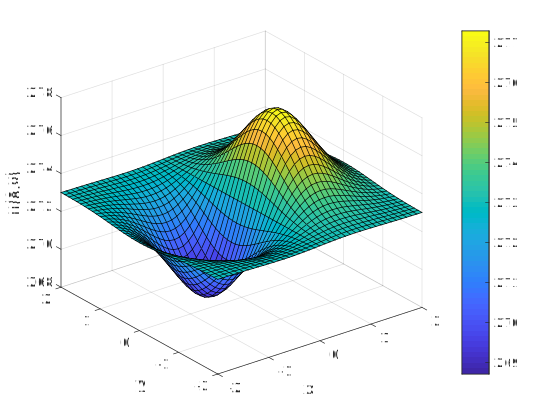
\includegraphics[width=0.7\linewidth]{../results/initial_condition_plot/initial_condition}
\caption{Grafické znázornění počáteční podmínky \eqref{eq:initial_condition}.}
\label{fig:initial_condition}
\end{figure}


\newpage{}

\bibliography{bib/Benes2017,bib/MMC}

%\bibliographystyle{plain}
\bibliographystyle{alpha}

\end{document}
